\vspace{0.5 cm}
\textcolor{blue} {\textit{Khadimoullah Vencatasamy}}
\vspace{0.3 cm}
\subsection{Trail Modelization}

We have define the secure zone with this equation:\\
\begin{equation}
\mathbb{X}(t)=\mathbb{G}\cap\mathbb{F}_\delta(\mathbb{X}(t-\delta))\cap\bigcap\limits_{i \leq}((g_(a_i))^-1(d_i(t),\infty)))\\
\end{equation}

Where $\mathbb{F}_\delta(\mathbb{X}(t-\delta))$ represents the past of the secure zone. In fact, we can associtae that to the trail of our robot. 
To compute the trail we have got to solutions. The first one was to stock the positions of our robot and then generate virtual robot with a smaller field of view. But with this solution we need to compute a lot ressources in interval analysis. So the second idea was to apply an erosion on an image. So we do not have to compute interval analysis. Then we give this new image with the trail to the script ImageToBoxes saving a lot of time of calculation.

\begin{figure}[H]
\begin{center}
  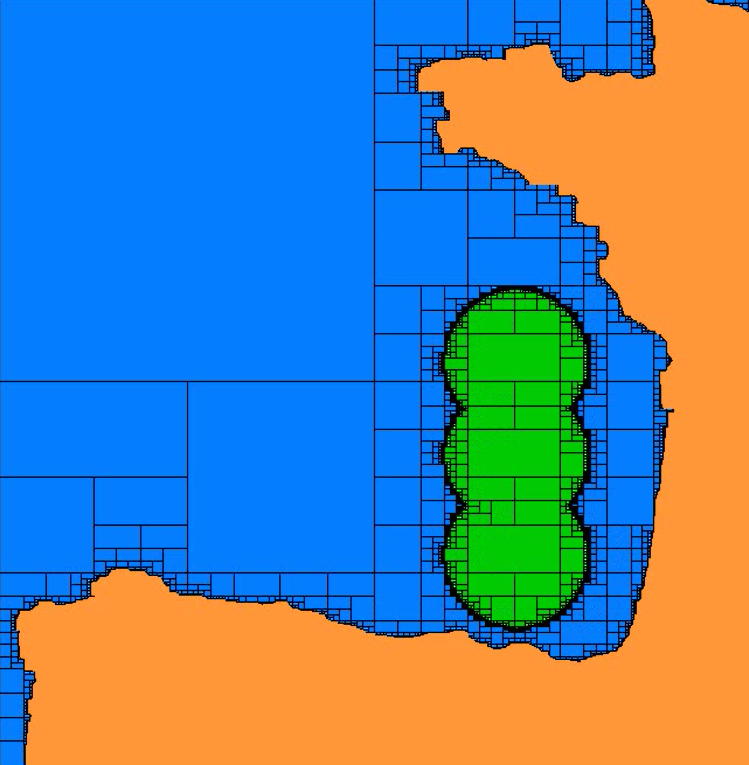
\includegraphics[width=0.6\linewidth]{WithoutTrail.png}
  \caption{Robot without}
\end{center}
\end{figure}


\begin{figure}
\begin{center}
  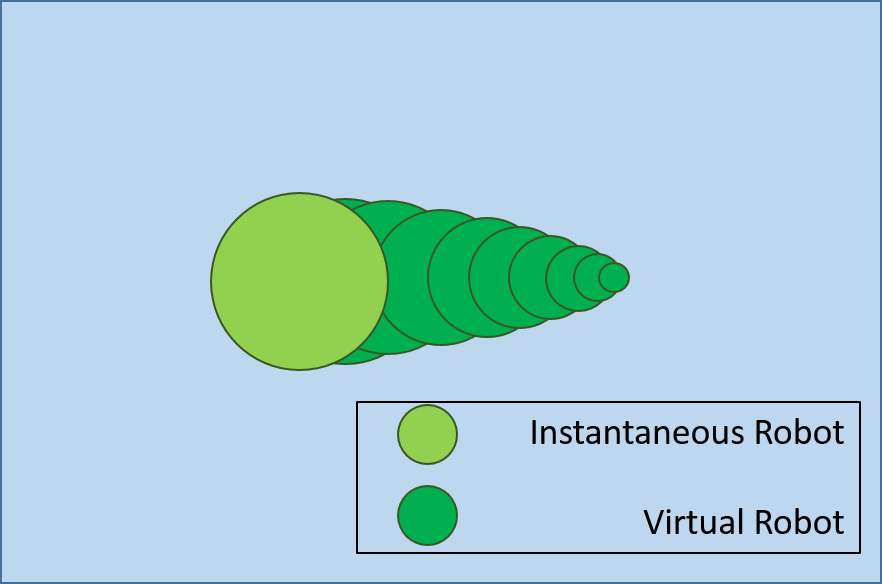
\includegraphics[width=0.6\linewidth]{TrailVirtualRobot.png}
  \caption{Trail Implementation with erosion}
\end{center}
\end{figure}

Finally, the erosion allow us to conclude if our algorithm is efficient. In fact, when the swarm covers the Bay of Biscay, even if a little zone is not covered the erosion will expand this area.

\begin{figure}[H]
\begin{center}
  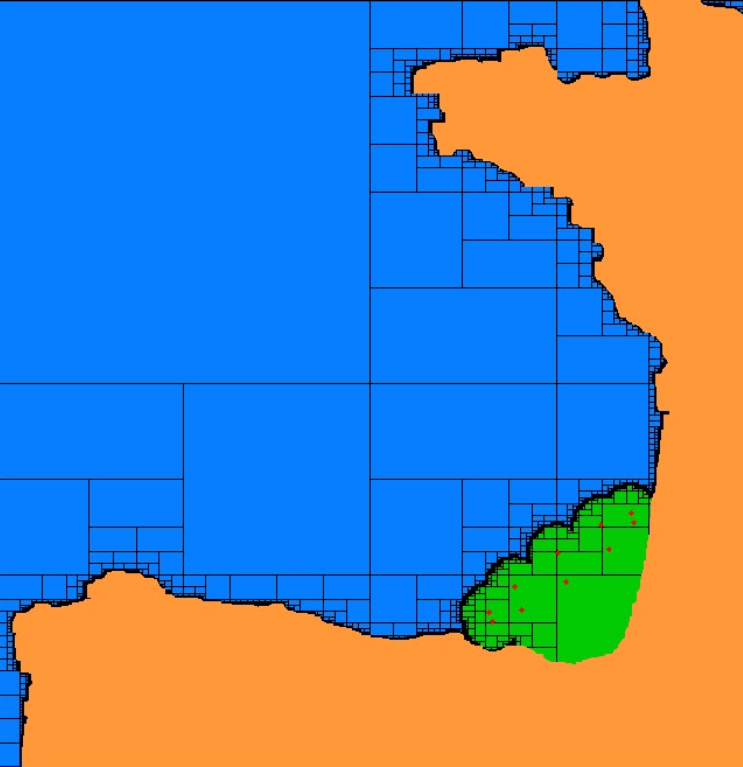
\includegraphics[width=0.6\linewidth]{FailZone.png}
  \caption{The swarm misses a little area}
\end{center}
\end{figure}

\begin{figure}
\begin{center}
  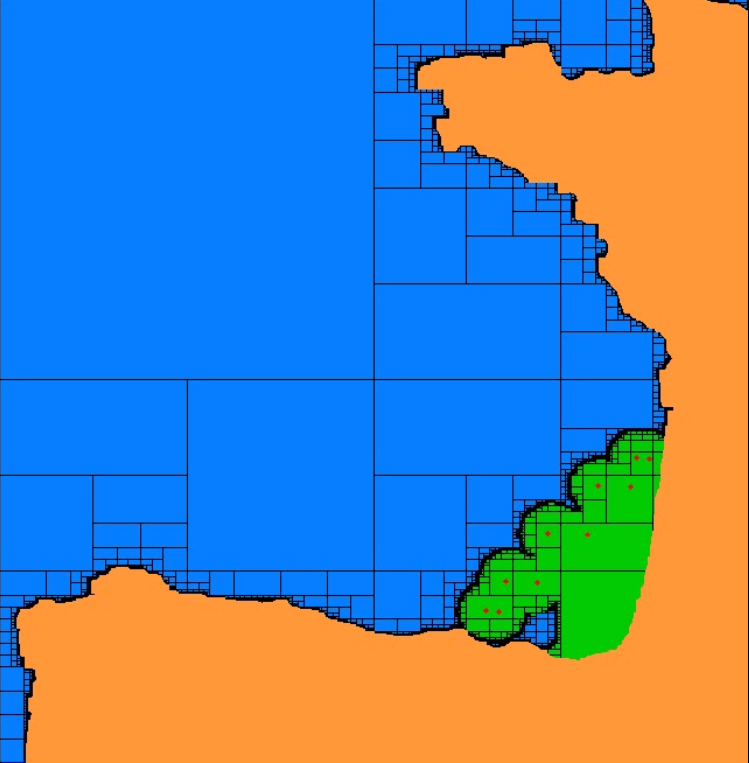
\includegraphics[width=0.6\linewidth]{FailZoneExpand.png}
  \caption{The uncovered area is expanded due to the erosion}
\end{center}
\end{figure}

